% Chapter3.tex
\chapter{WebDoc - Web Application Documentor}\label{ch:CP}

We have gone through the \textsc{Cinco} DSL specification for the graphical modeling tool, and now we will go over the editor created from it. We begin with a brief description of our graphical DSL, then demonstrate the critical building elements of our documentation architecture while simultaneously demonstrating our \textsc{Cinco} product: WebDoc\footnote{GitHub repository: \url{https://github.com/MukendiMputu/UserDoc}}. Next, we will show how to use these graphical elements to simulate a specific user workflow on the website we are documenting later. Finally, we demonstrate how to construct the target application that generates the Markdown files shown in the Web browser using the editor's built-in generator.

\begin{figure}[h]
    \centering
    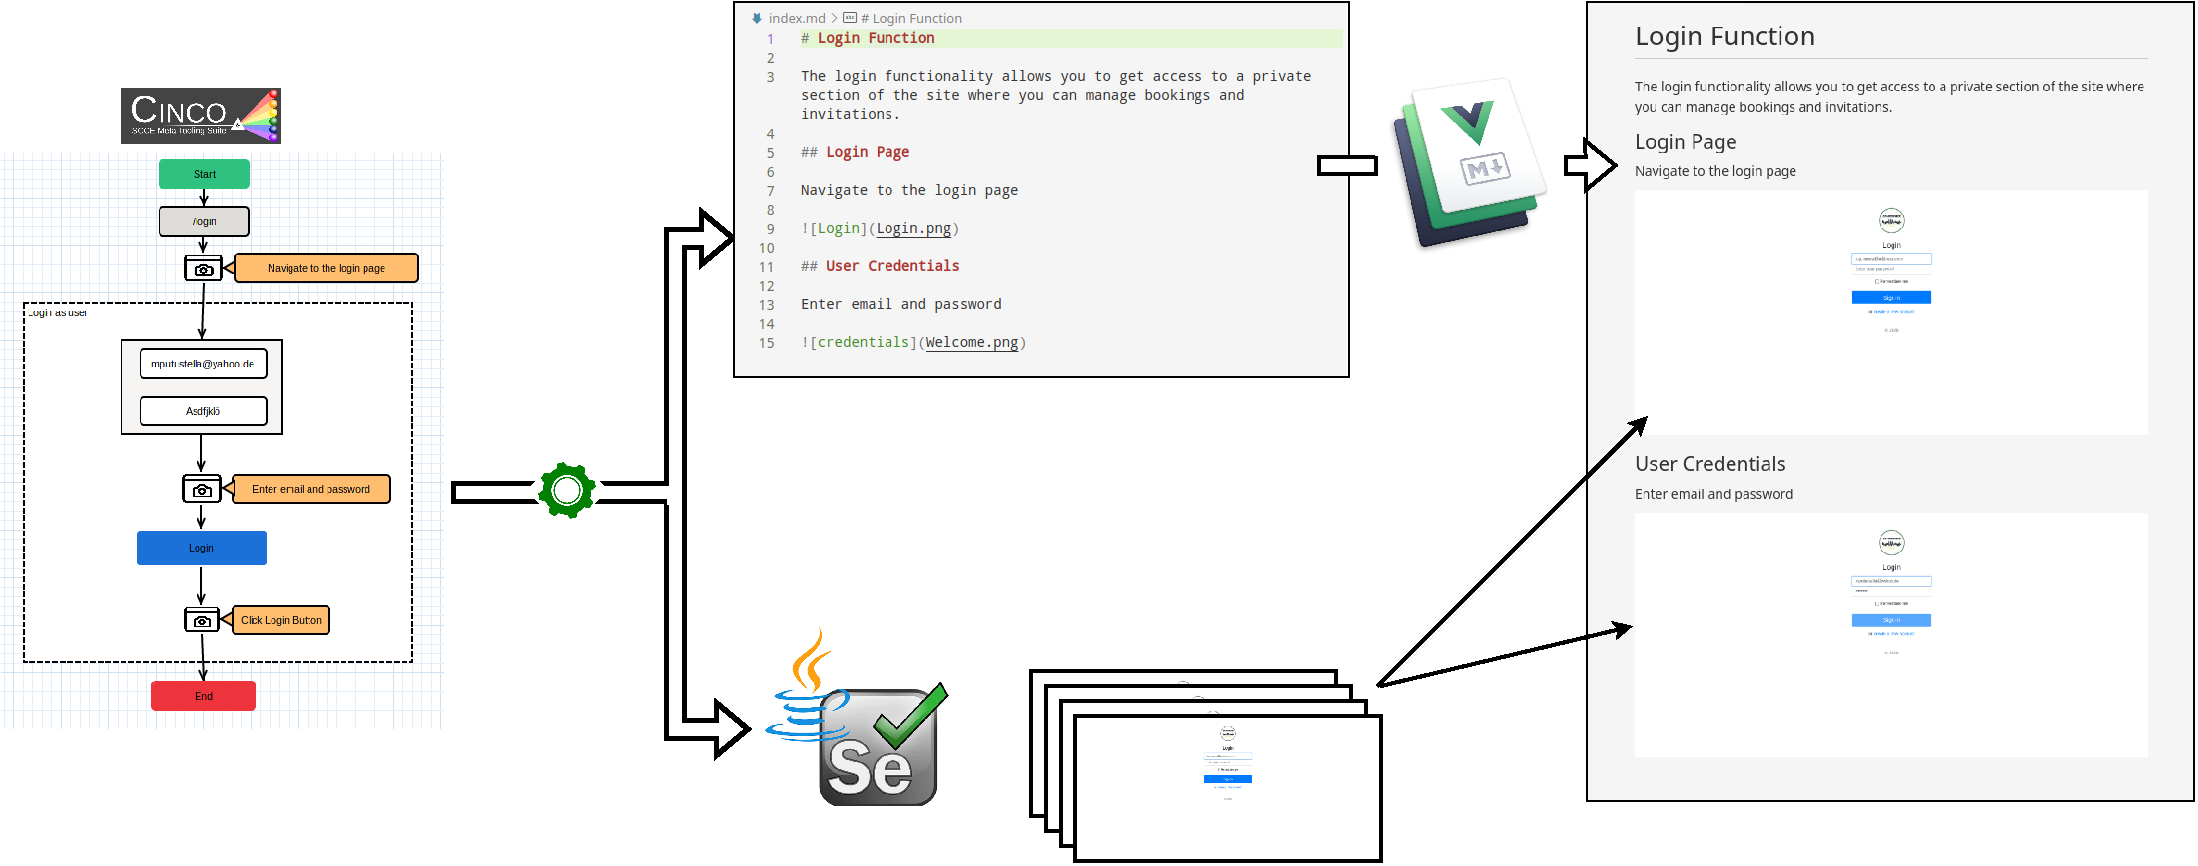
\includegraphics[width=\textwidth]{WebDoc-workflow.pdf}
    \caption{Generation process of End user Documentation}
    \label{fig:WebDocWorkflow}
\end{figure}

\section{Graphical DSL}\label{sec:gDSL}

Our graphical DSL primarily consists of node components with various appearances that match the actual Web items they represent to some extent and connector elements that connect the nodes to sequence graphs. This approximated replication aims to provide the developer with a sense of control over the interactable UI elements rather than replicating all potential Web elements. With those elements in hand, the designer can easily simulate a user activity by arranging nodes according to the Web application's navigation path. This graphical language is domain-specific because it is designed for modeling Web applications within a Web browser; for example, modeling documentation for a desktop application would be impossible.

\section{Graph Editor}\label{sec:graphEditor}

The WebDoc editor is mainly composed of the canvas in the middle of the working environment (1). The developer can drag and drop model elements from the palette on the right-hand side (2). Herein, elements are grouped into categories. On the left-hand side, we have the project explorer showing the current project structure (3). The main model files have the extensions .doc and .feat, where the latter is the entry point of the documentation application.

\begin{figure}[h]
    \centering
    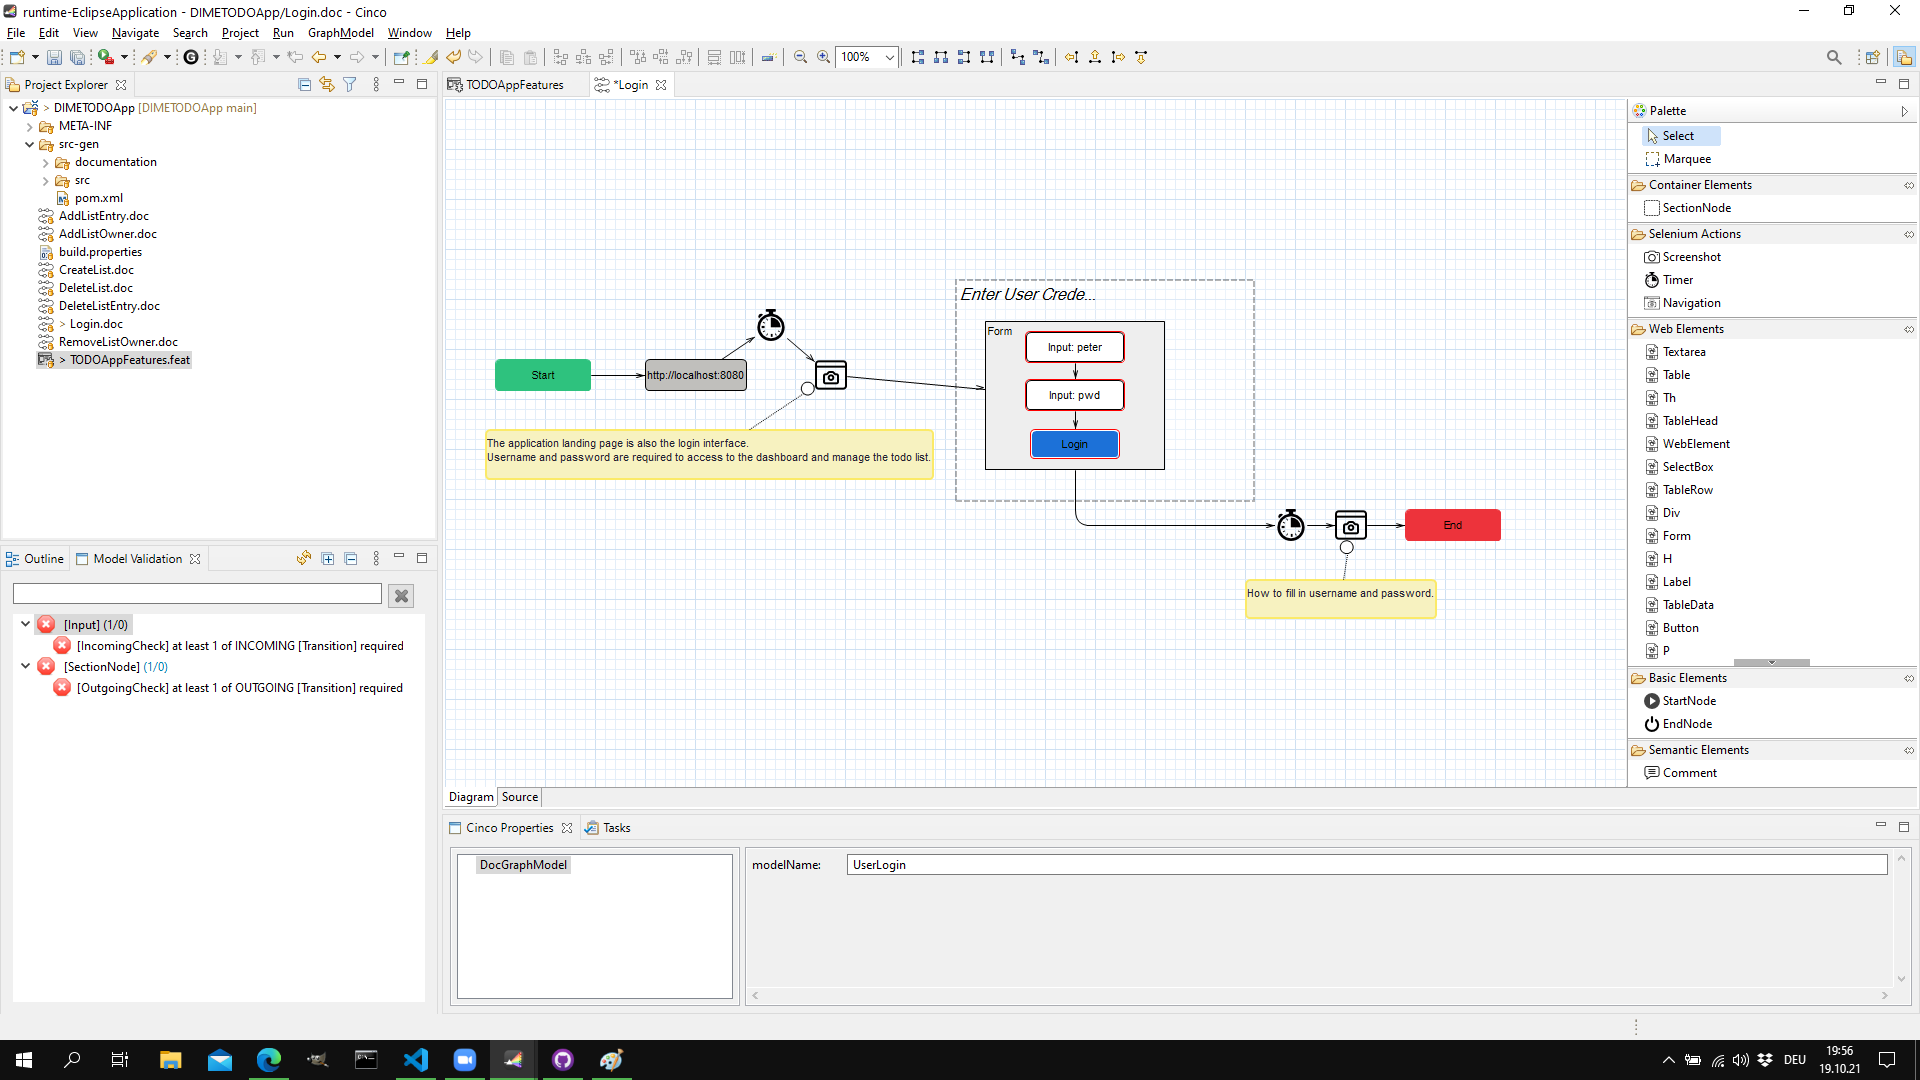
\includegraphics[width=\textwidth]{DocGraphModelChecks.png}
    \caption{\textsc{Cinco} Product Application - Graph model editor}\label{fig:graphDSL}
\end{figure}

All diagrams that are open in the editor are checked in the background for compliance with the requirements described on the metalevel and shown in the Model Checking view right beneath the project explorer (4). There is also the \textsc{Cinco} property view (5) that displays the attributes and values of any selected element in the editor. In this view, the developer can modify those values if the attribute field allows it.

\section{WebDoc's Model Elements}\label{sec:WebDocModelElem}

On a Web page rendered in the Web browser, there is a small amount of HTML elements the user can interact with. Most of them reside within the HTML forms, tools that are used for collecting data from the user or allowing them to control a user interface~\cite{mozillaMDN}. In addition, input fields (such as password, text area, checkbox) and buttons are prominent. Those are the Web elements that primarily constitute the palette of our model elements. In the previous chapter, we defined two different \glsplural*{mgl}: one for modeling the Web application features and the other one for modeling the user actions that make up those features.

\subsection{FeatureGraphModel}\label{sec:FeaGrahptModElem}

The FeatureGraphModel is the application starting point specified by the \lstinline{feature.mgl}. Here, the developer groups all the features that need to be documented in feature containers. For example, figure~\ref{fig:featGraph} shows a sample of the features modeled for our task management application, including the ability to log in, create a new list, add or remove a task from that list, and delete the entire list. The documentation website's resulting sidebar is depicted in Figure~\ref{fig:sidebar}, albeit the "Introduction" is not an application feature, instead the introductory page displaying the various functionalities. Moreover, our application offers the possibility also to add a new list owner already existing in the system as a regular user.

On the top left-hand corner, there is a property container holding the WebDriver property, whose value is set to \lstinline[language=MGL]{FIREFOX}. It is one of the additional model elements that help the developer define configurations that otherwise could not be modeled but are still essential for the execution of the application. This property value will be assigned to the Selenium WebDriver variable in the Java class. Remember that the executable file for the chosen WebDriver must already exist somewhere in the file system, and the path to it must be specified here in the property view.

\begin{figure}[H]
    \begin{subfigure}[b]{0.5\textwidth}
        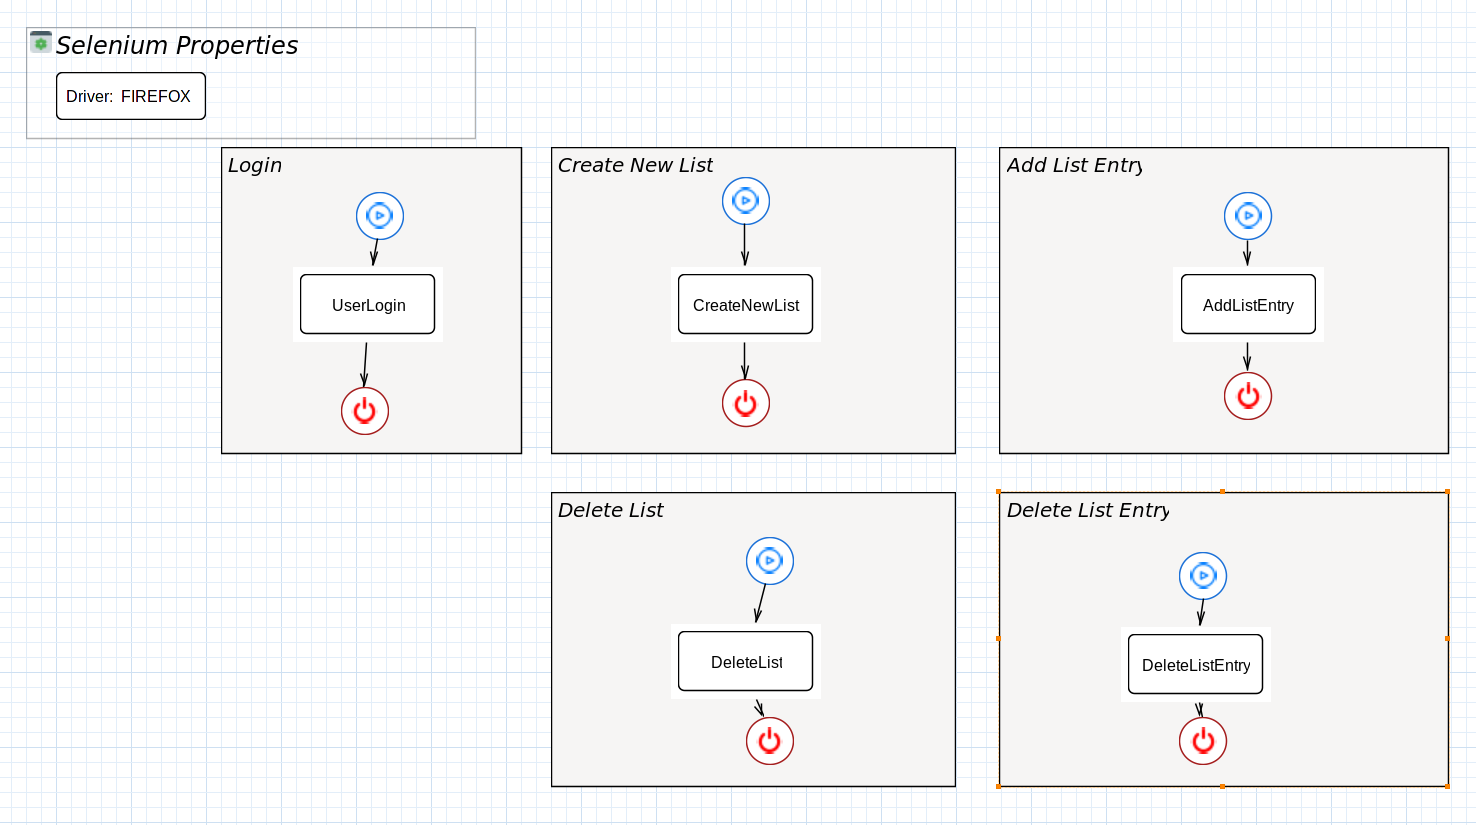
\includegraphics[width=\textwidth]{FeatureGraphModel2.png}
        \caption{Features in the FeatureGraphModel}
        \label{fig:featGraph}
    \end{subfigure}
    ~
    \begin{subfigure}[b]{0.5\textwidth}
        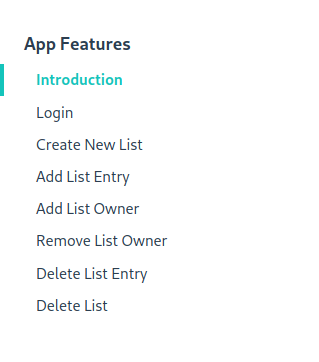
\includegraphics[width=\textwidth]{Sidebar.png}
        \caption{Menu structure on the documentation website}
        \label{fig:sidebar}
    \end{subfigure}
\end{figure}

Even though the features follow a logical workflow order, they are still distinct and generated separately. However, as indicated in the last chapter, this separation does not preclude reusability, as it is feasible to embed one whole DocGraphModel within another. Consider the CreateNewList functionality, which requires the user to sign in to create a new task list. Instead of repeating the login sequence in this one, the documentation developer may drag and drop the UserLogin.doc file into the diagram of the new model graph and connect it to the sequence as if it were a regular graph node. (see figure~\ref{fig:reusability}). Double-clicking on an imported subgraph sends straight to the original graph model. This double-click action was implemented by annotating the associated node specification with the \lstinline[language=MGL]{@doubleClickAction} annotation and providing a custom action class that holds the implementation logic. Furthermore, by unchecking the createScreenshots checkbox in the property view of a subgraph, the designer can disable the creation of screenshots for that specific model, which is enabled by default. This prevents the same screenshot from being taken several times when the subgraph is reused.

\begin{figure}[h]
    \centering
    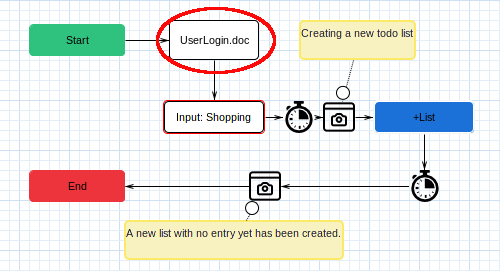
\includegraphics[width=0.75\textwidth]{Reusability.png}
    \caption{\textsc{Cinco} product - Reusing Login graph model in the CreateNewList graph model}
    \label{fig:reusability}
\end{figure}

The semantic elements in the feature graph model are incorporated into the underlying featureContainers for simplicity's sake. Clicking on a featureContainer opens the Cinco property view, which includes a multiline input form called 'description.' This is where the documentation designer can offer text content for the Markdown documentation files providing descriptive text for the diagram objects. These information texts will be gathered during the code creation process to create the complete documentation.

\subsection{DocGraphModel}\label{sec:DocGrahpModElem}

Figure~\ref{fig:loginSeq} illustrates the steps a user would take to log into our example Web application, as well as the Web elements that will be interacted with. They create the user login sequence for our Web application when connected in a logical sequence.

\begin{figure}[h]
    \centering
    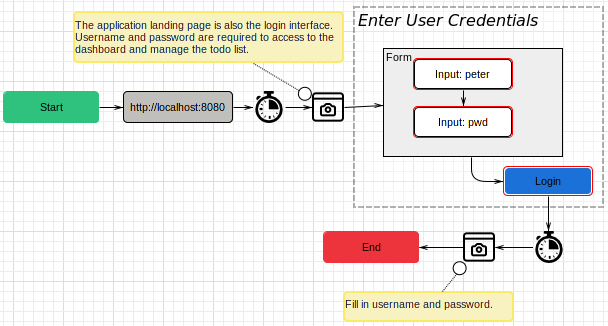
\includegraphics[width=0.85\textwidth]{WebDoc-graphModel.png}
    \caption{Example of a user workflow: here the login sequence}
    \label{fig:loginSeq}
\end{figure}

The sequence begins with the start node, which is the starting point of every user sequence, then comes the Navigation node used to navigate from one Web page to another. Next, the timer node waits explicitly for the number of seconds determined by the designer in the property view and for a certain condition to become true before continuing. Those ExpectedConditions are i.e., \lstinline{presenceOfElementLocated}, \lstinline{elementToBeClickable}, just to name a few. If we take, for example, the condition \lstinline{presenceOfElementLocated}, the timer holds the WebDriver execution for 3 seconds, checking every 500 milliseconds if the targeted Web element appears on the page. Because some items take time to load completely, this step is required for capturing all page elements when taking the screen capture. Right after the timer comes the Screenshot node that captures the current application state, displaying the application landing page, the login page. In the property view, one can give a unique file name to each image to be saved. The comment node allows the document writer to contribute descriptive information about the image that will later be appended to the Markdown file as an image caption. Next comes the Section node that regroups form elements for entering and validating user credentials. All input nodes, as well as the button node, have a red border that represents the highlighted state of the element. The model designer may see which elements will be highlighted in the following screenshot, after which the login sequence will end. 

The purpose of the Web element nodes is to allow the concrete \gls*{html} elements in the browser to be addressed. This implies that appropriate actions can be applied to such a representation of an \gls*{html} element. For instance, considering the input field in the picture below, the action of typing in a text is made possible by providing a property variable \lstinline{content}, whose value is then displayed inside the node element (i.e.,~''peter'' and ''pwd''). The same holds for button elements, which can be applied to the click action, or for select boxes, which can be dropped down to reveal the options they contain. In addition to that, all Web elements can be highlighted either by setting the \lstinline{highlighted} property to true or by letting the Highlight node under the \textit{Selenium Actions} category take care of it. The screenshot coming after will have that specific element surrounded with a red border as well (see fig.~\ref{fig:screenshot}).

\begin{figure}[h]
    \centering
    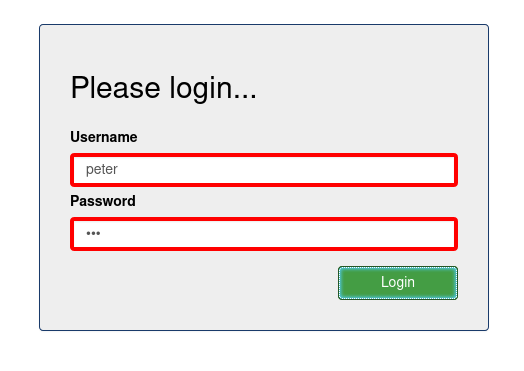
\includegraphics[width=0.55\textwidth]{ApplicationLandingPage.png}
    \caption{Login pane with screenshot of the highlighted input element}
    \label{fig:screenshot}
\end{figure}

In addition, each node element includes a description attribute, which, as discussed in the preceding section, provides additional content for Markdown files. We decided to hide this attribute in the property view to avoid overcrowding the diagram with semantic components describing each and every node member. All model diagrams are traversed during the generation process, and all descriptive texts are collected into paragraphs, then sections, and finally full Markdown files, depending on the feature they are included in. As a result, the documentation content is organized in the following fashion (see fig.~\ref{fig:markdown}): the featureContainer title is rendered as page headings, the DocGraphModel name is displayed as section headings with all other element descriptions underneath it, and so on.

\begin{figure}[h]
    \centering
    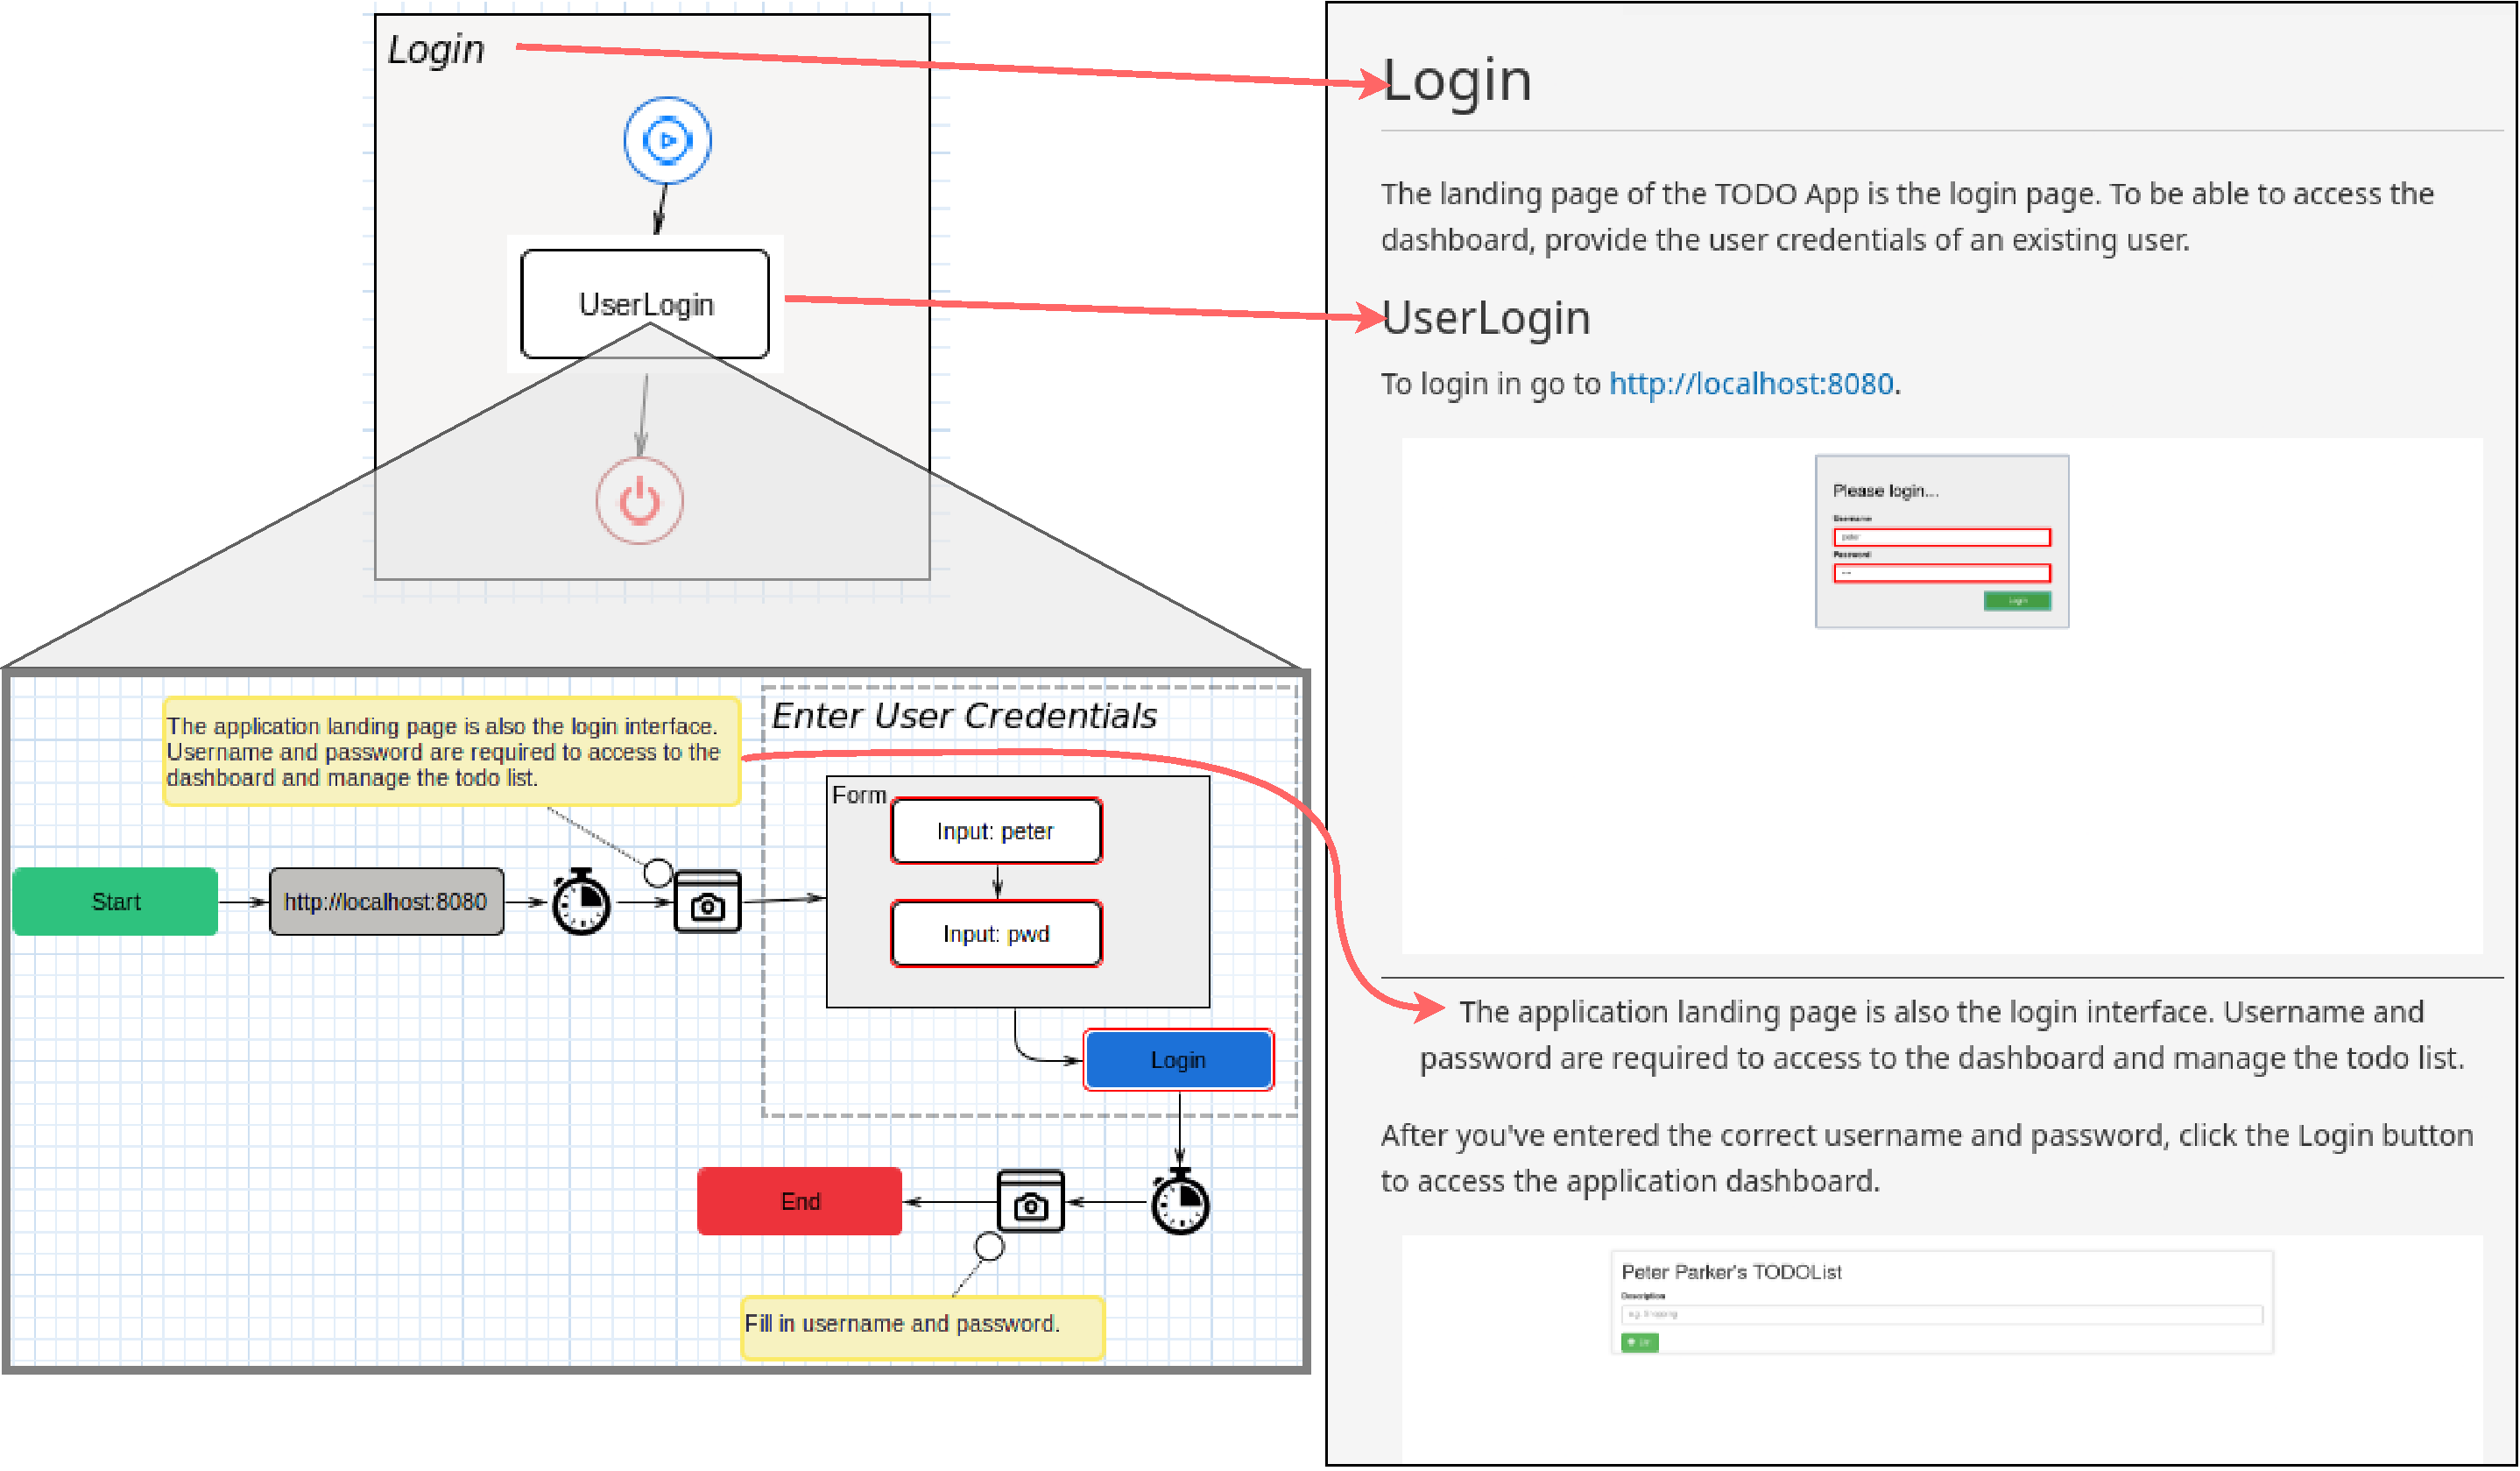
\includegraphics[width=\textwidth]{MardownStructure.pdf}
    \caption{Structural mapping of models to Markdown}
    \label{fig:markdown}
\end{figure}

\section{Graph Model Checks}\label{sec:modCheck}

Modeling functional graph diagrams is crucial for the correctness of the generated application code. Especially the Selenium-Java application code must correctly replicate the user sequence to capture the correct application state as the user would. This task is particularly daunting if the navigation graph of the underlying Web application is vast.

Therefore, we need to check that two distinct graph models do not have the same name or that for each user activity, there is a distinct path and no cycle inside that path.  These checks are reminiscent of various graph theory problems, such as determining whether a path from the start to the end node exists and whether a graph is cycle-free. The \textsc{Cinco} framework incorporates the MCaM plugin that does this operation~\cite{gitlabcinco}. specifying the \lstinline{@mcam("...")} or the \lstinline{@mcam_checkmodule("...")} annotation with the corresponding parameter in parentheses activates the plugin. Also, nodes and model graph attributes can be specified with the \lstinline[language=MGL]{unique} qualifier to enforce the uniqueness of the model name at design time.

\begin{figure}[h]
    \centering
    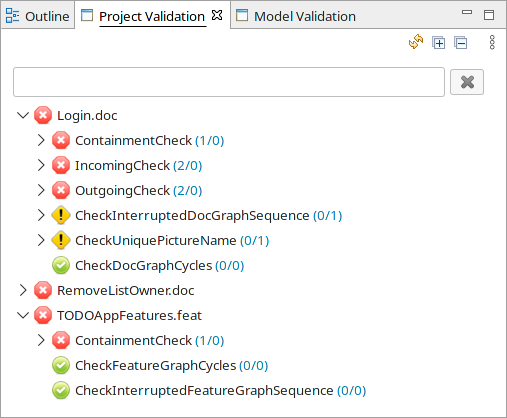
\includegraphics[width=0.7\textwidth]{ProjectValidationView.png}
    \caption{Project Validation view showing passed and failed checks}
    \label{fig:modelChecks}
\end{figure}

\subsection{MCaM Check}\label{sec:mcamCheck}

The first one must be declared right above the \lstinline[language=MGL]{graphModel} declaration with the parameter ''check''. It activates the check of the constraints on the graph nodes in the graph model scope. At design time, the model creator receives feedback shown as errors. Those mistakes either cause the generator to throw a runtime exception, or the resulting application code will be error-prone, hence, not executable. 

For this check to show a successful Incoming- or OutgoingCheck, the multiplicity of the relationship between node elements must respect the specified value. For example, a node element specified with an incoming Edge in this fashion \lstinline[language=MGL]{incomingEdges (Edge[1,*])}, must have at least one incoming connection of the \lstinline[language=MGL]{Edge} type. Any other kind of multiplicity can be defined; even not specifying any implies one. For instance, writing \lstinline[language=MGL]{incomingEdges (Edge)} is equivalent to \lstinline[language=MGL]{incomingEdges (Edge[*,*])}, which means at least and at most any number of \lstinline[language=MGL]{Edge} transition.

When specifying the containable elements of a container node (see i.e.~line~\ref{line:multiplicity} in listing~\ref{docMGL}), with the \lstinline[language=MGL]{containableElements} property, each elements listed in that property has a one type of multiplicity explained above. If not respected, the validation view will show a ContainmentCheck error until the designer resolves it.

\subsection{MCaM Module Check}\label{sec:mcamModCheck}

The second annotation allows us to specify our module checks. For instance, we need to ensure that two different screenshot nodes do not bear the same file name or that each sequence starts with the appropriate StartNode and ends with the EndNode. The first check makes sure that no screenshot overwrites another one that has the same name. The second one ensures that the resulting code reflects the model sequence from start to end. We also need to ensure that by integrating a DocGraphModel into another, we do not create cycles within the execution path. Otherwise, this would result in a never-ending execution loop once the generation process has started.

This module check allows us also i.e.~to check for unique feature names in the FeatureGraphModel scope. Although the featureContainers ensure the independence of each feature, two featureContainers bearing the same name would result in two documentation pages having the same title. The \textit{Project Validation} view shows all the checks done on the entire project and marks those that failed or passed the checks accordingly. Figure~\ref{fig:modelChecks} shows, for example, the checks done on our example project, where the Login.doc DocGraphModel passed the cycle check but failed the one checking for interruptions in the graph path and unique picture names.

\section{Generation Process}\label{sec:GenProcess}

After all of the essential models have been designed, the developer must generate executable code. Recall that we want to generate two different projects: the Selenium-Java project to capture the screenshots and the VuePress project containing all the documentation Markdown files. Therefore, we thought of two ways to reach the intended result.

The first one consists of generating the Selenium-Java application from our model graphs and, subsequently, when executing generated application, creates the VuePress project with all the documentation files as shown in fig.~\ref{fig:firstGenProcess}. This approach would imply letting Java take care of the generation process of the Markdown files and the creation of the needed screenshot. An erroneous generation of the Selenium-Java application will leave the designer with no tangible result at all. In this approach, the generated application becomes a single point of failure.

\begin{figure}[h]
    \centering
    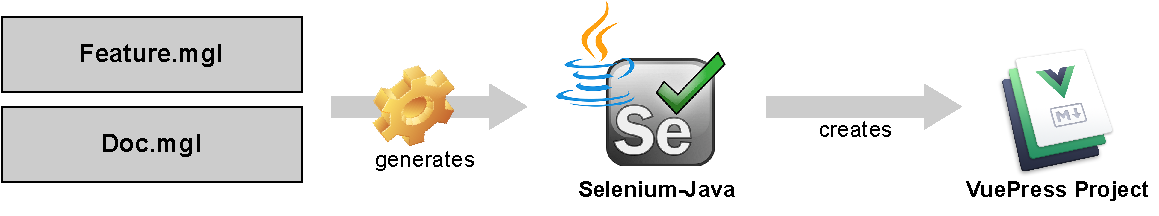
\includegraphics[width=\textwidth]{firstGenProcess.pdf}
    \caption{First approach: Sequential generation of the documentation}
    \label{fig:firstGenProcess}
\end{figure}

The second approach applies the concept of separation of concerns (see fig.~\ref{fig:secondGenProcess}). That means that we separate the task of taking screen captures with Selenium-Java from those generating the documentation files that will contain the screen captures. This way, if the Selenium-Java application contains errors that prevent taking screenshots, we can still generate a documentation website with placeholder pictures that can be later replaced with manually taken screen captures. It is almost apparent now that we opted for the second approach to create the documentation website.

So, clicking on the generate button creates an executable Selenium-Java application, which, once started, runs the user sequence model as a Selenium script in the Web browser. As mentioned in the preliminary chapter, the generator classes behind this process are Xtend classes. Xtend is a statically-typed programming language based on Java and translates to Java source code~\cite{Xtend}. 

\begin{figure}[h]
    \centering
    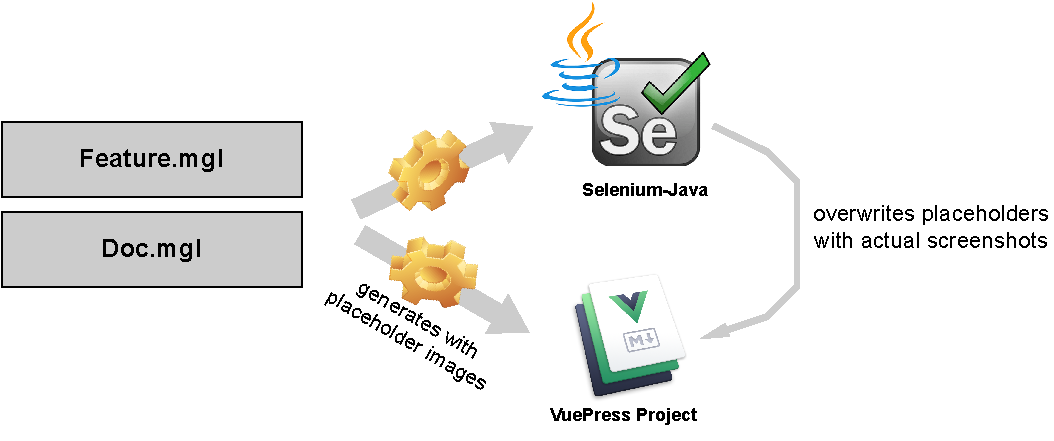
\includegraphics[width=\textwidth]{secondGenProcess.pdf}
    \caption{Second approach: Separate generation of the documentation}
    \label{fig:secondGenProcess}
\end{figure}

To start a generation process from a graph model, we must declare it ''generatable''. We do so by adding the \lstinline[language=MGL]{@generatable("path.to.generator.Class")} annotation in the graph model meta-specification. This annotation accepts as a parameter an Xtend or Java class that implements the IGenerator, whose \lstinline{generate} method starts the whole process and the path to a location where the generation product will be saved (in our case, it is in the \lstinline{src-gen} folder). We create two folder structures inside the src-gen folder: the first is the Java project structure with the Selenium script, and the second is the VuePress project holding all the Markdown files with the documentation text. Going deeper into technical details is beyond the scope of this paper; hence we illustrate the whole generation process in figure~\ref{fig:WebDocWorkflow}.
We begin by designing a graph model in the \textsc{Cinco} product application, the WebDoc editor; clicking on the generate button starts a simultaneous creation of both the project files mentioned earlier. At this point, the documentation pages are already available. We have chosen to generate the documentation file with references to placeholder pictures that will be overwritten once the Selenium script has been executed. After that, two simple commands are needed to launch the documentation website. Then again, we will not go deeper in details to stay in the scope of our thesis, but there is a great online guide on how to get started with VuePress~\cite{vuepress}. As for the Selenium-Java project, it can be imported in an \glsentryfull{ide} such as Eclipse and launched there. After successful execution, actual pictures overwrite all the placeholder and complete the documentation.